% Условная компиляция для самостоятельной работы
\ifdefined\mainfile
    % Если это часть основного файла, не добавляем начало и конец документа
\else
    \documentclass[12pt, a4paper]{report}
    \usepackage{/Users/vladbelousov/Desktop/Semestr_4-FP-NSU/Настройка/library}
    \usepackage[utf8]{inputenc} % Подключение поддержки UTF-8
    \begin{document}
\fi

%%-------------------------------%%

\chapter{Периодические решения}

\section{Периодические решения линейных систем}

\[ \frac{d}{dt } \vec{y }  = A(t ) \vec{y } + \vec{f } (t ) \quad  (1) \] 

\[ \vec{y}  (t ) =\begin{pmatrix}
y_1(t)\\
\vdots\\
y_n(t)
\end{pmatrix}  ,\quad  A(t ) = ( a_{ij }(t)  ) - (n \times  n) , \quad \vec{f} (t ) =\begin{pmatrix}
    f_1(t)\\
    \vdots\\
    f_n(t)
\end{pmatrix}  \] 
\[ a_{ij } (t ) \in C(\mathbb{R}) , \text{ } f_j (t ) \in  C(\mathbb{R} ) \Rightarrow \exists ! \text{ решение задачи Коши }  \begin{cases}
\displaystyle  \frac{d}{dt }  y = A (t ) y + f(t  ) \\
y(t_0 ) = t_0 
\end{cases} \]
\[ y(t )  \text{ - определенно при } t \in  \mathbb{R}\]   

\[ a_{ij }  (t+T      ) = a_{ij }  (t ) , \text{ }  \forall  t \in  \mathbb{R} , \text{ }  T > 0 \text{ - период}  \] 
\[ f_j (t + T ) = f_j(t)  \] 

Хотим узнать, существуют ли у системы (1) периодические решения, то есть \( \vec{y } (t+ T) = \vec{y } (t ) \).

\begin{theorem}
    Вектор функция \( \vec{y } (t ) \)  является \( T \)-периодическии решением системы (1) \( \Leftrightarrow  \vec{y } (0 ) = \vec{y }  (T)  \) 
\end{theorem}

\begin{proof} \(  \) 
    \begin{flushleft}
         \((\Rightarrow ): \text{ очевидно }  \)
    \end{flushleft}  

    \begin{flushleft}
        \( (\Leftarrow):  \) 
    \end{flushleft}

    Обозначим \( \vec{y } (0 )= \vec{y } (T )= \vec{y}  _0  \) 

    Рассмотрим задачу Коши \( \begin{aligned}
        \displaystyle \begin{cases}
            \displaystyle  \frac{d}{dt }  \vec{y }  = A(t ) \vec{y } + \vec{f }  (t)\\
            \vec{y } (0) = \vec{y } _0
            \end{cases}
            \quad \Rightarrow \exists  ! \text{ решение } \vec{y} (t ) 
    \end{aligned} \) 

    Рассмотрим функцию \( \vec{z } (t    ) = \vec{y } (t+T ) \) 

    \[ \begin{cases}
        \frac{d}{dt } \vec{z }  (t ) = \frac{d}{dt }  \vec{y }  (t +T) = \underbrace{A (t + T )}_{A(t )} \underbrace{\vec{y } (t+T )}_{\vec{z } (t )} +\underbrace{\vec{f }  (t + T )}_{\vec{f } (t )} \\
        \vec{z } (0) = \vec{y } (T ) = \vec{y } _0 
    \end{cases}\]  

\[  \text{, получим такую же задачу Коши}    \Rightarrow \vec{z } (t ) = \vec{y } (t ) \Rightarrow \vec{y } (t+T ) = \vec{y } (t)\] 
\end{proof}

\[ y ' = a(t ) y + f(t )\] 
\[ a(t +T ) = a(t ) \]  
\[ f(t+T ) = f(t )\]  

\begin{center}
    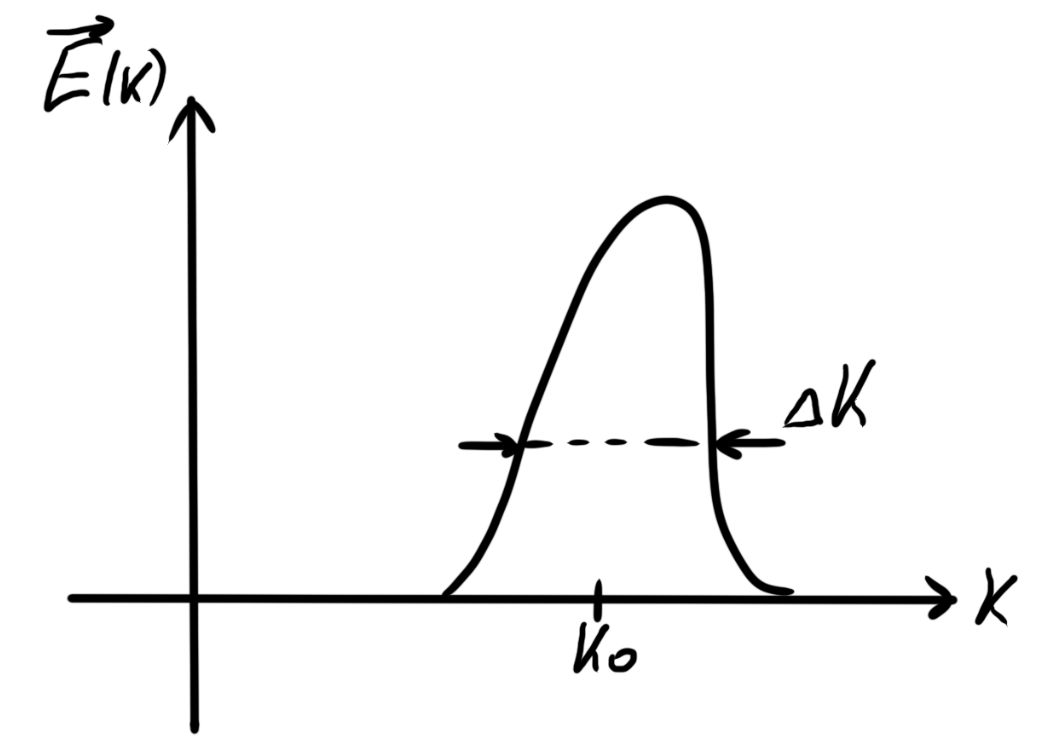
\includegraphics[width=0.4\textwidth]{/Users/vladbelousov/Desktop/Semestr_4-FP-NSU/ДфУ/Лекции_по_дням/image/30.png}
\end{center}

\begin{theorem}
    \( \exists !    \text{ }  T\)-периодическое решение системы (1) \( \Leftrightarrow  \det (\Phi (T ) - \Phi (0)) \neq 0  \), где \( \Phi(t) \) - ФМР системы \( \displaystyle  \frac{d}{dt } \vec{y } (t )= A(t )\vec{y} (t) \) 
\end{theorem}

\begin{proof}
    \begin{flushleft}
        Все решения системы \( \displaystyle  \vec{y }  (t) = \vec{ y } _{oo} (t )+ \vec{y } _{\text{ч} }(t ) = \Phi(t ) \vec{c }  + \Phi(t ) \cdot \int_{0}^{t }  \Phi^{-1 } (s ) \vec{f } (s )ds   \) 
    \end{flushleft}

    По теореме 1. : \( \vec{y } (0) = \vec{y } (T )  \):

    \[\Phi(0 ) \vec{c }  + \Phi(0 ) \int_{0 }^{0 } \Phi^{-1 } (s ) \vec{f } (s ) ds = \Phi(T ) \vec{c }  +\Phi(T ) \int_{0}^{T } \Phi^{-1 }  (s) \vec{f } (s ) ds  \] 

    \[\Phi ( 0) \vec{c } = \Phi (T ) \vec{c }  + \Phi (T ) \int_{0 }^{T }  \Phi^{-1 }  (s ) \vec{f } (s ) ds   \] 
    \[ (\Phi(0 )- \Phi(T ))\vec{c }  = \Phi(T ) \int_{0 }^{T } \Phi^{-1 } (s )\vec{f } (s )ds \Leftrightarrow  B \vec{c }  = \vec{\psi}  \]  

    \[ \exists ! \text{ } T\text{-периодическое решение  } \Leftrightarrow \exists ! \text{ }  \vec{c }  \Leftrightarrow  \det  (\Phi(0 )- \Phi(T )) \neq 0  \] 
\end{proof}

\begin{flushleft}
    \textbf{Замечание. } \textit{Если \( \det  B = \det  (\Phi(0 )- \Phi(T ))  = 0\), то}
    
    \textit{1) \( \rank B  = \rank  (B|\vec{\psi} ) \), то \( \exists \infty   \)  много \( T \)-периодических решений } 
    
    \textit{2) \( \rank B \neq  \rank (B|\vec{\psi} ) \), то не существует \( T \)-периодических решений. } 
\end{flushleft}

\begin{theorem}
    Пусть \(  A(t ) = A\) - постоянная матрица , \( \lambda_1, \ldots, \lambda_n \) - собственные числа \( A  \) \( \exists ! T \)-периодическое решение системы (1) \( \Leftrightarrow  \forall  \lambda_j \) выполняется \( e^{\lambda_j T } \neq 1  \) 
\end{theorem}

\begin{flushleft}
    \textbf{Замечание. } \textit{ \( e^{ \lambda_j T } \neq 1 \Leftrightarrow  \lambda_j T \neq 2 \pi k i , \text{ } k \in  \mathbb{Z} \) }  
\end{flushleft}

\begin{proof} \(  \) 
    \begin{flushleft}
        Если \( A(t ) = A \), то \( \Phi (t ) = e^{ t A} \)  
    \end{flushleft}

    Из теоремы 2. \( \exists  !  \text{ }  T  \) -периодическое решение \( \Leftrightarrow  \det (e^{TA }  -E ) = 0 \)
    
    \[ \mu_1, \ldots, \mu_n - \text{ собственные числа матрицы } e^{TA} \Rightarrow \forall  \mu_j \text{ } \mu_j \neq 1    \] 

    \[ A = S  YS^{-1} = , \text{ }  e^{TA }  = Se^{TY } S^{-1}   \] 
    \[ Y= \begin{pmatrix}
    \lambda_1 & ... & 0\\
    \vdots & \ddots &     \vdots\\
    0& ... & \lambda_n
    \end{pmatrix} ,\quad  e^{ TY } = \begin{pmatrix}
        e^{\lambda_1 T}  & ... & 0\\
        \vdots & \ddots &     \vdots\\
        0& ... & e^{\lambda_nT} 
        \end{pmatrix} \Rightarrow \mu_j = e^{\lambda_j T}   \] 
\end{proof}


\section{Периодические решения для линейных уравнений высокого порядка }

\[ y^{(n )} + a_{n-1 } (t )y^{(n-1 )} + ...+ a_1(t )y ' + a_0 y = f(t )  \quad  (2)\] 
\[ a_j(t ) , \text{ } f(t ) \in C(\mathbb{R} ) , \quad  a_j (t+T ) = a_j(t ) ,\quad  f(t+T ) = f(t ) , \text{  } t \in \mathbb{R} \] 

Цель: найти решение \( y(t ) : y(t+T )= y(t )\)

\begin{theorem}
    Функция \( y(t) \) является \( T \)-периодическим решением уравнения (2) \( \Leftrightarrow  y(0 ) = y(T )  ,\text{ } y'(0 ) = y'(T ) ,..., y^{(n-1 )} (0 ) = y^{(n-1)}(T)  \)  
\end{theorem}

\begin{proof} \(  \) 
\begin{flushleft}
    \( (\Rightarrow): \) 
\end{flushleft}

Дано:  
\[  y(t+T )= y(t ) , \text{ }  t \in \mathbb{R}  \] 
\[ y'(t+T ) = y' (t) \]  
\[ \vdots \] 
\[ y^{(n-1 )} (t+T ) = y^{(n-1 )}  (t) \] 
\[ \Rightarrow t =0 \Rightarrow \text{ получаем требуемое}  \] 

\begin{flushleft}
    \( (\Leftarrow): \) 
\end{flushleft}

Сведем уравнение к системе: 

\[ \begin{cases}
y_1 = y \\ 
y_2 = y' \\ 
\vdots \\ 
y_n = y^{(n-1)} 
\end{cases} \]

\[ \frac{d}{dt} \begin{pmatrix}
y_1 \\
y_2\\
\vdots\\
y_n
\end{pmatrix} = \underbrace{\begin{pmatrix}
    0 & 1 & 0 & ... & 0\\
    0 & 0 & 1 & ... & 0\\
    &  &  & \ddots & \\
    0 & ... & ... & ... & 1\\
    -a_0  & -a_1  & ... & ... & -a_{n-1} 
    \end{pmatrix}}_{A_n(t)}\begin{pmatrix}
    y_1 \\
    y_2\\
    \vdots\\
    y_n
\end{pmatrix} + \begin{pmatrix}
    0 \\
    0\\
    \vdots\\
    f_n
\end{pmatrix} \quad (3) \] 

\[ y_1 (0 )= y_1 (T  ) ,\quad  y_2 (0 ) =y_2 (T ) ,..., y_n (0 ) = y_n (T) \] 

\[ \begin{aligned}
    (3):\begin{cases}
        \displaystyle  \frac{d}{dt } \vec{y }  = A_n (t )\vec{y } + \vec{f } (t ) \\ 
        \vec{y } (0 ) = \vec{y } (T)
    \end{cases}
    \quad \Rightarrow \text{ по теореме 1. }  \vec{y } (t +T ) = \vec{y } (t )
\end{aligned} \] 

В частности, \( y_1 (t +T ) = y_1 (t ) \) 



\end{proof}

\begin{theorem}
    \( \exists  ! \text{ }  T  \)-периодическое решение уравнения (2) \( \Leftrightarrow  \det  (\Phi (T ) - \Phi (0))\neq 0  \), где \( \Phi (t) \) - ФМР однородной системы (3), то есть: 

    \[ \Phi(t ) = \begin{pmatrix}
    \varphi_1 (t) & ... & \varphi_n(t)\\
    \varphi_1 '(t)& ... &  \varphi_n '(t)\\
     \vdots&  & \vdots\\
     \varphi_1^{(n-1)} (t) & ... &  \varphi_n^{(n-1)} (t)
    \end{pmatrix} , \quad  \{\varphi_1 (t ), ..., \varphi_n (t)\}  \text{ - ФСР для однородного уравнения (2)} \] 
\end{theorem}

\textit{
    Доказательство следует из теоремы 2. } 

\begin{theorem}
    Пусть \( a_j(t ) = a_j  \)  - постоянные коэффициенты. Рассмотрим характеристическое уравнение: \( \lambda^n + a_{n -1 } \lambda^{n-1 }  +...+ a_1 \lambda + a_0 =0  \text{  }  ,\lambda_1, \ldots, \lambda_n  \) - его корни. \( \exists ! \text{  } T \)-периодическое решение уравнения (2) \( \Leftrightarrow  \forall  \lambda_j  \) выполняется \( e^{\lambda_j T } \neq 1   \) 
\end{theorem}

\begin{proof} \(  \) 

    \begin{flushleft}
        Сведем уравнение     к системе, получим систему (3). 

        По теореме 3. \( \exists ! \text{ } T \)-периодическое решение системы (3) \( \Leftrightarrow  \forall  \lambda_j (A_n) \)-собственные числа матрицы \( A \) выполняется \( e^{\lambda_j T}  \neq 1  \)   
    \end{flushleft}
В прошлом семестре: \( \det  (A_n - \lambda E) = (-1 )^{n }  [\lambda^n + a_{n-1 }  \lambda^{n-1 }  +...+ a_1 \lambda + a_0] \) 
\[  \] 
\end{proof}

\section{Нахождение периодических решений с помощью рядов Фурье}

\[ y '' + \alpha y ' + \beta y = f(t ) \quad (4) \] 
\[ \alpha, \text{ }  \beta \in  \mathbb{R}   , \text{ } f(t  ) \in C(\mathbb{R} ) , \text{ }  f(t+T ) = f(t ) , \text{ }  t \in \mathbb{R} \] 
\[ f(t ) \text{ - кусочно-гладкая} \]  

\[ f(t ) = \frac{a_0}{2 }  + \sum_{k =1}^{\infty  }\left( a_k \cos \left( \frac{2 \pi}{T } kt   \right) + b_k \sin  \left( \frac{ 2\pi }{T } kt   \right) \right)   \]  
\[ a_k = \frac{2}{T }  \int_{0}^{T } f(t ) \cos \left( \frac{2\pi }{T } kt   \right)dt , \quad  b_k = \frac{2}{T }  \int_{0 }^{T }  f(t )\sin \left( \frac{2 \pi }{T }kt   \right)  dt \] 

Замена \( \displaystyle  \frac{ 2 \pi }{T } t = s \Leftrightarrow  t = \frac{T}{2 \pi } s :   \) 

\[ f(t ) = f\left( \frac{T}{2 \pi }s   \right)   = \tilde{f } (s ) = \tilde{f }\left( \frac{2\pi }{T }t  \right)\]  
\[ \underbrace{f(t +T )}_{f(t )=\tilde{f }(s)} =\tilde{ f } \left( \frac{ 2\pi }{T} (t +T ) \right) = \tilde{ f } \left( \frac{2\pi }{T } t + 2 \pi   \right)  = \tilde{ f } (s + 2 \pi)\]  

\[ y(t )= y \left( \frac{T}{2 \pi } s   \right)  = \tilde{ y }(s ) = \tilde{y }\left( \frac{2\pi}{T}t  \right)\]  
\[ y '(t ) = \frac{d}{dt  }  \tilde{y }(s ) = \frac{d}{ds }  \tilde{ y }(s ) \frac{ds}{dt } = \tilde{y }' (s ) \cdot \frac{2\pi}{T} \]  
\[ y''(t ) = \tilde{y }'' (s ) \left( \frac{2\pi}{T}  \right) ^2 \]  

\[ (4 ) \Leftrightarrow  \tilde{y }'' ( s )\left(  \frac{2\pi}{T }  \right) ^2 + \alpha \tilde{ y }' (s  ) \cdot \frac{2\pi}{T} + \beta \tilde{y }(s ) = \tilde{f}(s ) \Leftrightarrow  \tilde{ y }'' (s ) + \alpha \tilde{ \alpha }\tilde{y }' (s )+ \tilde{\beta} \tilde{y }(s ) = \tilde{\tilde{f }} \] 
\[ \tilde{\tilde{f }}(s+ 2 \pi) = \tilde{\tilde{f }}(s) \] 


%%-------------------------------%%

% Закрытие документа, если файл компилируется отдельно
\ifdefined\mainfile
    % Если это основной файл, не нужно заканчивать документ
\else
    \end{document}
\fi